%-------------------------------------------------------------------------------
% File: main.tex
%       Compile using:
%           $ pdflatex main.tex
%           $ biber main
%
% Author: Marco Pinna
%         Created on 08/04/2022
%-------------------------------------------------------------------------------
\documentclass[11pt, a4paper, twoside, openany]{book}

% equal left and right margins
\usepackage[hmarginratio=1:1]{geometry}

% configuration to typeset documents in english
\usepackage[english]{babel}
\usepackage{import}
% include graphics in the file
\usepackage{graphicx}
\usepackage{pgf}
\usepackage{tikz}
% used in the dedication environment definition
\usepackage{afterpage}

% used to set page background image
\usepackage{tikz}

% used to handle math equations and formulas
\usepackage{amsmath}
\usepackage{mathtools}
\usepackage{array}

% used to handle quotes
\usepackage{csquotes}

%used to handle bibliography
\usepackage[backend=bibtex,
style=alphabetic,
citestyle=authoryear
]{biblatex}
\addbibresource{references.bib}

%used to change color and background color of single words
\usepackage{xcolor}

%used to place figures side by side
\usepackage{subfig}

%used to fix figure positioning
\usepackage{float}

%used to reference sections
\usepackage{hyperref}

\usepackage{wrapfig}

\usepackage{blkarray}

\usepackage{hyperref}
% for itemize with leftmargint parameter
\usepackage{enumitem}

% blank page command
\newcommand{\blankpage}
{
    \null
    \thispagestyle{empty}%
    \addtocounter{page}{-1}%
    \newpage
}
\newcommand\inputpgf[2]{{
\let\pgfimageWithoutPath\pgfimage
\renewcommand{\pgfimage}[2][]{\pgfimageWithoutPath[##1]{#1/##2}}
%\input{#1/#2}
}}
% dedication environment
\newenvironment{dedication}
{
    % blank page before dedication
    \afterpage{\blankpage}
    % we want a new page
    \clearpage
    % no header and footer
    \thispagestyle{empty}
    % some space at the top
    \vspace*{\stretch{1}}
    % the text is in italics
    \itshape
    % flush to the right margin
    \raggedleft
    % blank page after dedication
    \afterpage{\blankpage}
}
{
    % end the paragraph
    \par
    % space at bottom is one times that at the top
    \vspace{\stretch{1}}
    % finish off the page
    \clearpage
}

\newenvironment{specifications}
{
	\fontfamily{qtm}\selectfont
}{\par}


%-------------------------------------------------------------------------------
% Title page
%-------------------------------------------------------------------------------
\title{
    \vspace{-3cm}
    
\includegraphics[scale=0.3]{img/cherubino_black.eps}\\
    {\scshape {\huge University of Pisa}}\\
    MSc in Computer Engineering\\
    \rule{7cm}{0.01cm}\\
    {\large{\scshape Electronics and Communication Systems}}\\
    [2cm]
    {\scshape Design and implementation of a CRC algorithm on a Xilinx Zynq Board}\\
    [3cm]
	    
    
    \LARGE{\textbf{Supervisors}\hfill\textbf{Student}}\\
    \Large{\emph{Prof. Luca Fanucci}\hfill\emph{Marco Pinna\\}}
    \Large{\emph{Prof. Massimiliano Donati}\hfill\emph{\hphantom{.}\\}}
    \Large{\emph{Ing. Pietro Nannipieri}\hfill\emph{\hphantom{.}\\}}
    \vfill
    \date{\today}
}

% leave the author field ampty in the title page
\author{}


\begin{document}
\maketitle

% blank page before dedication
\afterpage{\blankpage}	

% enable page numbering back: roman numbers style
\pagenumbering{roman}

% print table of contents
\tableofcontents

% set arabic page numbering style
\pagenumbering{arabic}

%-------------------------------------------------------------------------------
% File: specifications.tex
%
% Author: Marco Pinna
%         Created on 08/04/2022
%-------------------------------------------------------------------------------
\chapter*{Specifications}
In what follows, the design and implementation of a CRC algorithm on a Xilinx Zynq Board is carried out.\\
The specifications are the following (translated from Italian):
\hfill \break
\begin{displayquote}
    \begin{specifications}
    {\Large Implementation of a CRC algorithm}\\
		Design a digital circuit that implements the Cyclic Redundancy Check (CRC) algorithm, both for the \textit{sender} and for the \textit{receiver}, according to the specifications below.
		Such algorithm is a powerful control method that exploits the idea of redundancy; a sequence of F redundant bits (Frame Control Sequence FCS)is added (by the sender) to a data sequence M, so that the transmitted message, on M+F bit, is divisible by a predefined divisor called CRC polynomial. The receiver, through a division by the same polynomial used by the sender, can detect the correctness of the received data.\\
\\
	Message M=56 bits\\
	Frame Control Sequence F=8 bits\\
	CRC polynomial of degree 9: $x^{8} + x^{4} + x^3 + x^{2} + 1$\\
	(The binary representation of the polynomial will therefore be 100011101)\\
	Transmitted message M+F=64 bit
	
		
		
		\begin{figure}[H]
		    \begin{center}
	        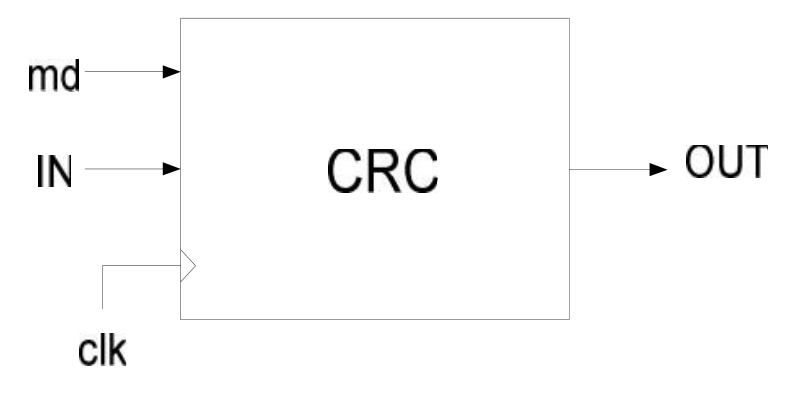
\includegraphics[scale=0.5]{img/high_lvl_schematics.png}

        	\label{fig:high_lvl_schematics}
    		\end{center}
    	\vspace*{-0.4cm}
\end{figure}

Through the \texttt{md} signal one can set whether the circuit is to be used as sender or as receiver.\\
When operating as receiver the last F values of OUT indicate the correctness of the received message.\\
\\
\\
\underline{The final project report has to include}:
\begin{itemize}
	\item Introduction (description of the algorithm, possible applications, possible architectures, etc.)
	\item Description of the architecture selected for the realization (block diagram, inputs/outputs, etc.)
	\item VHDL code (with detailed comments)
	\item Test-plan and relative testbench for verification
	\item Results of the automated logic synthesis on Xilinx FPGA Zync platform: resources used (slice, LUT, etc.), maximum operating frequency, critical path, etc. commenting potential warning messages
	\item Conclusions
\end{itemize}
    \end{specifications}
\end{displayquote}
%-------------------------------------------------------------------------------
% File: introduction.tex
%
% Author: Marco Pinna
%         Created on 08/04/2022
%-------------------------------------------------------------------------------
\chapter{Introduction}\label{ch:introduction}
The work is organized as follows:
\begin{itemize}
	\item this chapter contains the description of the algorithm, some of its applications and possible architectures for the implementation
	\item in chapter \ref{ch:architecture} an in-depth explanation of the chosen architectures is given
	\item in chapter \ref{ch:vhdl_code} the VHDL code of each component is shown and commented
	\item chapter \ref{ch:testplan} concerns the test plan and the testbenches used for the verification of the system
	\item chapter \ref{ch:synth_results} shows the results of the automated logic synthesis on the Xilinx FPGA Zync platform
	\item finally in chapter \ref{ch:conclusions} conclusions are drawn and some consideration about possible optimizations or different implementations are made
\end{itemize}

\section{Algorithm description}\label{sec:alg_description}
A Cyclic Redundancy Check (CRC) algorithm is a technique used in digital networks that uses redundant bits to detect accidental changes in digital data.\\
Let us supposed to have a \textit{sender} (S) and a \textit{receiver} (R) at the two end of a communication channel.\\
To each message M of \texttt{m} bits being sent by S, an additional section (the Frame Control Sequence, or FCS) of \texttt{f} redundant bits is added, whose value is computed performing a polynomial division between the message M (the dividend) and a polynomial G (the divisor) called \textit{generator} and calculating the remainder of such division.\\
Upon reception, R performs the same division and, depending on the value of the remainder, it is able to check whether the message M has been corrupted during transmission.\\

\noindent More in detail:
\begin{itemize}[leftmargin=0pt, topsep=0pt,itemsep=-1ex,partopsep=1ex,parsep=1ex]
	\item[-] let $M$ be an \texttt{m} bits long binary string.\\
	An \texttt{m-1} degree polynomial $M(x)$ is associated to it, such that the \textit{i}-th coefficient of the polynomial is equal to the \textit{i}-th bit of the string (e.g. $100101111 \Rightarrow x^{8} + x^{5} + x^{3} + x^{2} + x + 1$).\\
	\item[-] Let $G(x)$ be the generator polynomial whose binary representation is \texttt{f + 1} bits long (the degree of G(x) will therefore be \texttt{f}).\\
M is shifted to the left by \texttt{f} positions, padding to the right with \texttt{f} zeros. This corresponds to multiplying $M(x)$ by $x^f$.\\
	\item[-] The FCS is built as follows:\\
	a polynomial \textit{long division} between $x^{f}{\cdot}M(x)$ and $G(x)$ is performed, using finite field arithmetic on the Galois Field GF(2). Let $Q(x)$ and $R(X)$ be the quotient and the remainder of such division, respectively. \\
	It follows that 
	\begin{equation}
		x^{f}{\cdot}M(x) = Q(x)\cdot G(x) + R(x)
		\label{eq:polynomial1}
	\end{equation}
\\
	If we subtract $R(x)$ from both sides of the equation, we get
	\begin{equation}
			x^{f}{\cdot}M(x) - R(x) = Q(x)\cdot G(x)
			\label{eq:polynomial2}
	\end{equation}
	\item[-] The polynomial on the left-hand side of the equation is divisible by $G(x)$ and contains the original message M in the \texttt{m} highest bits and the FCS in the \texttt{f} lower bits (by construction, the degree of $R(X)$ is strictly less than \texttt{f}, so it can be represented on \texttt{f }bits).\\
	\item[-] This \texttt{m+f} bits long string M{$|$}FCS is what will be sent to the receiver.\\
	\item[-] The receiver can check the integrity of the message by dividing M{$|$}FCS by $G(x)$ and checking whether the remainder is equal to 0: if it is, then the message M has likely not been corrupted during transmission, otherwise it has and thus needs to be discarded.
\end{itemize}
\hfill \break
In this particular implementation, M will be 56 bits long, the generator will be

	\begin{equation}
		\begin{split}
			x^{8} + x^{4} + x^{3} + x^{2} + 1
	  	\end{split}
	\quad\leftrightarrow\quad
  		\begin{split}
			100011101
  		\end{split}
	\label{eq:generator}
	\end{equation}
therefore the FCS will be 8 bits long, for a total of 64 bits to be sent for each message.
\paragraph{Example}
\mbox{}\\
Let us use as an example the transmission of the word ``hi'' encoded in ASCII.\\
The binary string corresponding to ``hi'' is:
	\begin{equation}
	01101000\:\:01101001
	\label{eq:example_binary}	
	\end{equation}
We first pad it with zeros
	\begin{equation}
	01101000\:\:01101001\:\:00000000
	\label{eq:example_padded}	
	\end{equation}
then we compute the FCS by performing the long division between \ref{eq:example_padded} and \ref{eq:generator}.\\

\newdimen\digitwidth
\settowidth\digitwidth{0}
\def~{\hspace{\digitwidth}}


\def\divrule#1#2{%
\noalign{\moveright#1\digitwidth%
\vbox{\hrule width#2\digitwidth}}}
\begin{tabular}[b]{@{}r@{}}
\begin{tabular}[t]{@{}l@{}}
011010000110100100000000\\
~100011101\\
\divrule{1}{9}
~0101111001\\
~~100011101\\
\divrule{2}{9}
~~00110010001\\
~~~~100011101\\
\divrule{4}{9}
~~~~0100011000\\
~~~~~100011101\\
\divrule{5}{9}
~~~~~000000101010000\\
~~~~~~~~~~~100011101\\
\divrule{11}{9}
~~~~~~~~~~~00100110100\\
~~~~~~~~~~~~~100011101\\
\divrule{13}{9}
~~~~~~~~~~~~~000\textbf{10100100}\\
\end{tabular}
\end{tabular}
\\
\hfill \break
The remainder R is $10100100$. R is subtracted from (\ref{eq:example_padded}) to create the FCS in the 8 lower bits, yielding the following string

	\begin{equation}
	01101000\:\:01101001\:\:10100100 .
	\label{eq:example_with_FCS}	
	\end{equation}


\section{Possible applications}\label{sec:possible_applications}
CRC algorithms are used extensively in various data transmission technologies and protocols: SATA, USB, Ethernet, CDMA, Bluetooth, etc.\\
They are also found in several standards, programs and file formats such as MPEG-2, PNG, Gzip, to name a few.\\
There are different implementations of CRC algorithms, each with its own polynomial. The choice of the polynomial (both its degree and its coefficients) depend on several factors such as the maximum desired overhead and the sensitivity to different errors.\\

\noindent An important remark to be made is that such algorithms protect against \textit{accidental} corruption of data, but they are not suited against \textit{intentional} alteration of data, since a valid CRC to attach to the tampered message can easily be computed once the algorithm is known.

\section{Possible architectures}\label{sec:possible_architectures}
Two different architectures were identified to implement the algorithm:
\begin{itemize}
\item the first one simply implements the long division shown in \ref{sec:alg_description} using shift registers, accumulators, counters , XOR gates, etc.\\
In this implementation the algorithm advances bit by bit, therefore in order to ``consume" the whole message (56 bits), a total of at least 56 clock cycles is needed.
\item the second one exploits the facts that the divisor (i.e. the generator) is fixed and that in GF(2) there is no carry, therefore adjacent bytes have no influence on each other during the algorithm. It is then possible to pre-compute the division for each possible byte and store the results in a LUT.\\
This allows to perform the division byte by byte, thus speeding up the whole process. This solution will be more efficient in terms of speed, at the expense of a greater use of resources on the FPGA since a 256x1B LUT has to be created.
\end{itemize}
%-------------------------------------------------------------------------------
% File: architecture.tex
%
% Author: Marco Pinna
%         Created on <date>
%-------------------------------------------------------------------------------
\chapter{Architecture}\label{ch:architecture}

%TODO add intro of chapter


%-------------------------------------------------------------------------------
% File: vhdl_code.tex
%
% Author: Marco Pinna
%         Created on 16/04/2022
%-------------------------------------------------------------------------------
\chapter{VHDL code}\label{ch:vhdl_code}
This chapter consists of an in-depth analysis of the VHDL codebase of the project, commenting the more interesting parts and providing the reasons behind the development choices that were made.\\
While the initial development process followed a top-down approach to find the most appropriate architecture(s) and identify the components, the actual coding process followed a \textbf{bottom-up} approach, starting from the simplest components and basic units and going up to build progressively more complex modules.\\
As mentioned in chapter \ref{ch:architecture}, the development process was carried out with modularity in mind: this allowed to ease the reuse of components and simplify debugging and maintenance. Furthermore, some well-known VHDL best practices were followed, especially for naming signals, constants and modules.\\
\hfill \break
The directory structure of the project is the following:\\
\dirtree{%
.1 CRC.
.2 modelsim.
.2 src.
.3 DFF.vhd.
.3 DFF\_N.vhd.
.3 D2FF.vhd.
.3 D2FF\_N.vhd.
.3 PIPOShiftReg.vhd.
.3 xor\_logical.vhd.
.3 xor\_LUT.vhd.
.3 control\_unit/.
%.4 fullAdder.vhd.
%.4 rippleCarryAdder.vhd.
%.4 counter.vhd.
%.4 controlUnit\_bitwise.vhd.
%.4 controlUnit\_LUT.vhd.
.3 CRC\_bitwise.vhd.
.3 CRC\_LUT.vhd.
.2 tb.
.2 vivado.
}

\pagebreak

In order not to clutter the document too much, only the most important parts of each source file will be displayed here. The complete source files can be found in the project repository linked in chapter \ref{ch:introduction}.\\


\section{D2FF}\label{section:D2FF.vhd}
\lstset{style=codestyle}\label{code:D2FF.vhd}
\lstinputlisting[language=VHDL,caption={VHDL source code of D2FF}]{code/D2FF.vhd}
\hfill \break
As \ref{code:D2FF.vhd} shows, the source for D2FF is quite simple and very similar to a typical description of a classic D Flip Flop: the only difference is the presence of an additional \texttt{if..else} statement needed to multiplex the two input data signal by means of the \texttt{sel} input.\\

\section{D2FF-N}\label{code:D2FF_N.vhd}
The D2FF-N source code is exactly the same as the D2FF, except for the type of the input ports \texttt{d0} and \texttt{d1} and the output port \texttt{q}, which are all declared as \texttt{std\_logic\_vector}s and the presence of a \texttt{generic} which allows to size the component to suit one's needs.

\section{PIPO Shift Register}\label{sec:PIPOShiftReg.vhd}
\lstset{style=codestyle}\label{code:PIPOShiftReg.vhd}
\lstinputlisting[language=VHDL,caption={VHDL source code of the PIPO Shift Register}]{code/PIPOShiftReg.vhd}
\hfill \break
Listing \ref{code:PIPOShiftReg.vhd} shows the source code for the PIPO Shift Register. As mentioned in \ref{subsec:PIPOshiftreg}, its building unit is the D2FF. The presence of the generic \texttt{ShiftLen} at line 4 made this component suitable for both the chosen architectures: \texttt{ShiftLen} will be equal to 1 for the bitwise logic and it will be equal to 8 for the bytewise logic.\\
The port maps at lines 32 and 45 to the \texttt{en} input of the D2FF are set to \texttt{1} since in neither of the architectures there is the need to stop the shifting.\\
%If one were to add the handshake mechanism mentioned at the end of chapter \ref{ch:architecture}, the \texttt{en} could be controlled by an expanded Control Unit that would then be able to pause and resume the shifting.

\section{XOR logical}\label{sec:XOR_logical.vhd}
\lstset{style=codestyle}\label{code:XOR_logical.vhd}
\lstinputlisting[language=VHDL,caption={VHDL source code of the XOR logical component}]{code/XOR_logical.vhd}
\hfill \break
The \textbf{XOR\_logical} component is a combinatorial component which implements a single subtraction step needed for the polynomial long division procedure.\\
It computes the XOR between the 8 least significant bits of the input and the generator. As mentioned in \ref{sec:bitwise_arch}, the input most significant bit is used as an ``enable", i.e. when it is \texttt{0} the circuit simply outputs the input 8 least significant bit. This is implemented in line 17 by exploiting the fact that \texttt{0} is the neutral element of the XOR operation.\\

\section{XOR LUT}\label{sec:XOR_LUT.vhd}
\lstset{style=codestyle}\label{code:XOR_LUT.vhd}
\lstinputlisting[language=VHDL,caption={VHDL source code of the XOR LUT component}]{code/XOR_LUT.vhd}
\hfill \break
The \textbf{XOR\_LUT} component is again a combinatorial component which contains a look-up table for the specified generator polynomial.\\
It computes the XOR between the 8 least significant bits of the input and the generator. The input is converted into an integer and then used as an index to retrieve the corresponding entry of the LUT.\\
Since the input is 8 bits long and so are the output, the total size of the LUT is 256 B.\\
The LUT was generated with a simple Python script.
\pagebreak
\section{Control Unit}\label{sec:control_unit.vhd}

\dirtree{%
.1 CRC/src/control\_unit/.
.2 fullAdder.vhd.
.2 rippleCarryAdder.vhd.
.2 counter.vhd.
.2 controlUnit.vhd.
}
\hfill \break
The \texttt{control\_unit} directory contains the source code for the Control Unit along with the subcomponent it is made of.\\
The source code of the \textbf{full adder} and the \textbf{ripple-carry adder} will not be shown here since they are both very simple.

\subsection{Counter}\label{subsec:counter.vhd}
\lstset{style=codestyle}\label{code:counter.vhd}
\lstinputlisting[language=VHDL,caption={VHDL source code of the Counter}]{code/counter.vhd}
\hfill \break
Listing \ref{code:counter.vhd} shows the VHDL source code for the Counter.\\
It is made of a ripple-carry adder, a register of D Flip-Flop and some logic to wrap the count back to 0 when the maximum value is reached.\\
As with the PIPO Shift Register, this Counter also has a generic which allows the user to set the max count. When instancing a Control Unit component (v. next subsection), this will also have a generic for the number of cycles; this generic will be inherited by the Counter generic. %TODO rephrase? improve?
\\
\pagebreak
\subsection{Control Unit}\label{subsec:controlUnit.vhd}
\lstset{style=codestyle}\label{code:controlUnit.vhd}
\lstinputlisting[language=VHDL,caption={VHDL source code of the Control Unit}]{code/controlUnit.vhd}
Listing \ref{code:controlUnit.vhd} shows the VHDL source code of the Control Unit.\\
Thanks to the generic \texttt{CU\_cycles}, both the CRC architectures can use the same \textit{ControlUnit} component, by just changing the generic map upon instantiation.\\
This was made possible by avoiding the so-called ``magic numbers" in the code and by noticing that all the phases can be defined in terms of the same offsets with respect to the start or the end of the computation, regardless of the architecture.
\pagebreak

\section{Bitwise CRC}\label{sec:CRCbitwise.vhd}
\lstset{style=codestyle}\label{code:CRC_bitwise.vhd}
\lstinputlisting[language=VHDL,caption={VHDL source code of the bitwise architecture of the CRC}]{code/CRC_bitwise.vhd}
\hfill \break
Listing \ref{code:CRC_bitwise.vhd} shows the VHDL source code of the bitwise architecture of the CRC. Components and constants declarations were omitted to avoid cluttering, as well as the clock and reset mapping for each component. Please refer to the repository for the full source code.\\
The structure of the CRC source code is actually quite straightforward, as it mainly consists of the previously shown subcomponents and signals that interconnect them.\\
The \texttt{mux\_proc} process at line 123, as the name suggests, implements the multiplexing process that feeds the 8 least significant bits into the shift register, depending on the value of \texttt{MD}.\\
The signal assignments at the end of the architecture use the concatenation operator \texttt{\&} to implement the ``merging" of the signals.

\section{LUT-based CRC}\label{sec:CRC_LUT.vhd}
Given the strong similarity of the LUT-based CRC implementation with respect to the bitwise one, below is a highly reduced version of VHDL source code of the former, which only contains the parts that differ from listing \ref{code:CRC_bitwise.vhd}.\\
It is worth mentioning that the CRC ``interface" (i.e. the set of input and output ports) is obviously the same in both architectures and compliant with the project specifications.

\lstset{style=codestyle}\label{code:CRC_LUT.vhd}
\lstinputlisting[language=VHDL,caption={VHDL source code of the LUT-based architecture of the CRC}]{code/CRC_LUT.vhd}
\hfill \break
As listing \ref{code:CRC_LUT.vhd} shows, the only few differences with the bitwise version are some minor changes in the size of some signals and registers, the presence of the \textbf{XOR\_LUT} combinatorial block in place of the previously used \textbf{XOR\_logical} and the assignment to the \texttt{accum\_d1} signal at line 54. At each step, the next input of the accumulator consists of the bitwise XOR between the appropriate LUT entry and the next byte in the message.
%-------------------------------------------------------------------------------
% File: testplan.tex
%
% Author: Marco Pinna
%         Created on <date>
%-------------------------------------------------------------------------------
\chapter{Test-plan and testbench}\label{ch:testplan}
The design of each component was followed by a testing phase performed via testbench modules, also written in VHDL, to ensure that said component was designed properly. Only the testbench of the final CRC modules will be presented in this chapter. Please refer to the repository for the rest of them.\\
\hfill \break
All the simulations of the testbenches were performed on \textit{ModelSim - Intel FPGA Starter Edition v. 2020.1}.\\

\section{CRC testbench}
As mentioned in \ref{sec:CRC_LUT.vhd}, the set of input and output ports of the CRC is the same, regardless of the implementation, because of the compliance with the specifications. This naturally led to a single testbench that could test both versions.\\
\hfill \break
A Python script was used to generate 10 random 7 bytes long messages and compute the CRC of each of them.
\begin{itemize}
	\setlength{\itemsep}{1pt}
  	\setlength{\parskip}{0pt}
  	\setlength{\parsep}{0pt}
	\item[-] \texttt{0526abfa59289d 75}
	\item[-] \texttt{1ad743298a5b0c 13}
	\item[-] \texttt{49dbf2d3fca778 7a}
	\item[-] \texttt{58de7943c3b4e1 f7}
	\item[-] \texttt{7a32768bdb8fb4 58}
	\item[-] \texttt{8d73243271fdf2 86}
	\item[-] \texttt{c387f7b71ddd50 2e}
	\item[-] \texttt{d8c66625791098 b7}
	\item[-] \texttt{e34a300fa4c345 1d}
	\item[-] \texttt{f9e70f4d2b6ed3 89}
\end{itemize}
\pagebreak
The testbench consists of three phases:
\begin{itemize}
	\item sender mode
	\item receiver mode with intact messages and correct CRCs
	\item receiver mode with corrupted messages
\end{itemize}
During the first phase \texttt{MD} is equal to \texttt{0} and the 10 random messages are input in succession. The output should show each of the 10 messages, in succession, and the correct CRC as the least significant byte.\\
During the second phase, \texttt{MD} is equal to \texttt{1} and the input consists of the 10 random messages each with its own CRC attached, in succession. The output should show each of the 10 messages, in succession, and the least significant byte equal to \texttt{0x00}.
The third phase is equal to the second phase, except for the output which should show non-zero values, proving the error detecting properties of the CRC algorithm.\\
Below are some screenshots from the testing phase on Modelsim.\\

\begin{figure}[H]
    \begin{center}
        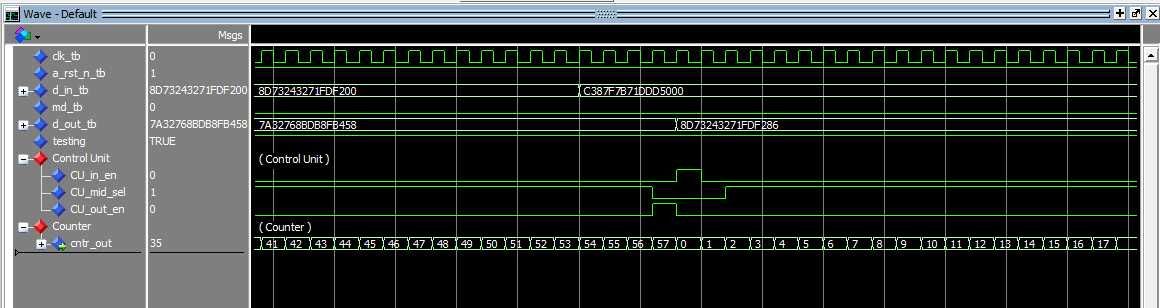
\includegraphics[scale=.6,clip]{img/test_bit_phase1.png}
    \end{center}
    \vspace*{-0.5cm}
    \caption{Testbench simulation of the bitwise architecture (phase 1)}
    \label{fig:test_bit_phase1}
\end{figure}

\begin{figure}[H]
    \begin{center}
        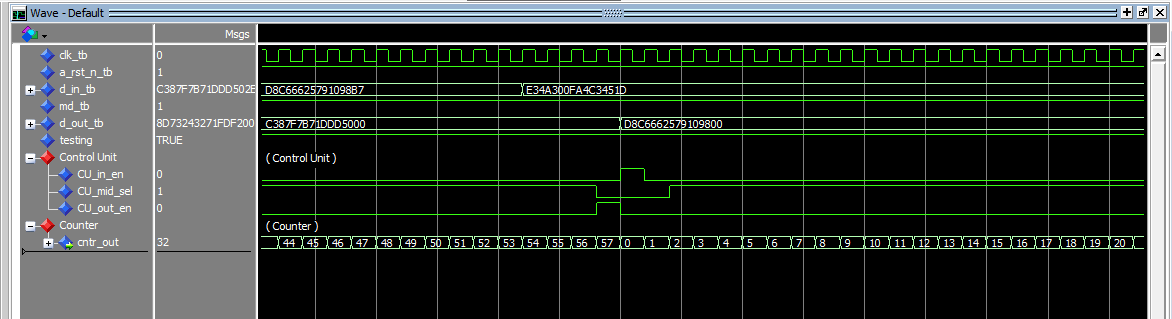
\includegraphics[scale=.6,clip]{img/test_bit_phase2.png}
    \end{center}
    \vspace*{-0.5cm}
    \caption{Testbench simulation of the bitwise architecture (phase 2)}
    \label{fig:test_bit_phase2}
\end{figure}

\begin{figure}[H]
    \begin{center}
        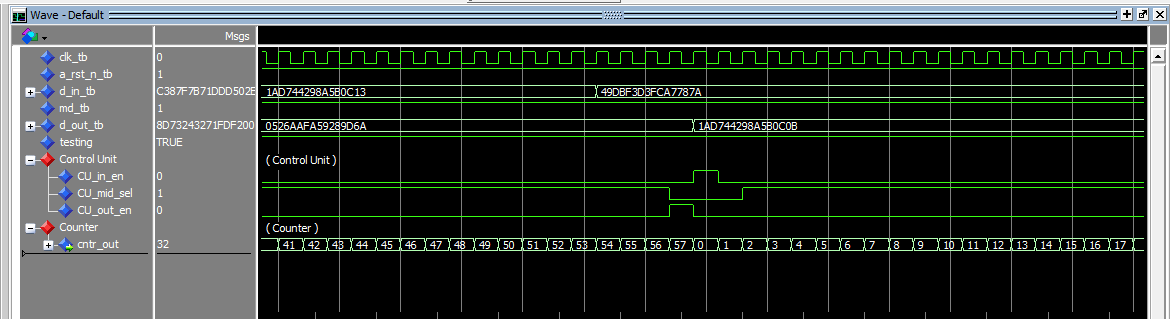
\includegraphics[scale=.6,clip]{img/test_bit_phase3.png}
    \end{center}
    \vspace*{-0.5cm}
    \caption{Testbench simulation of the bitwise architecture (phase 3)}
    \label{fig:test_bit_phase3}
\end{figure}

\begin{figure}[H]
    \begin{center}
        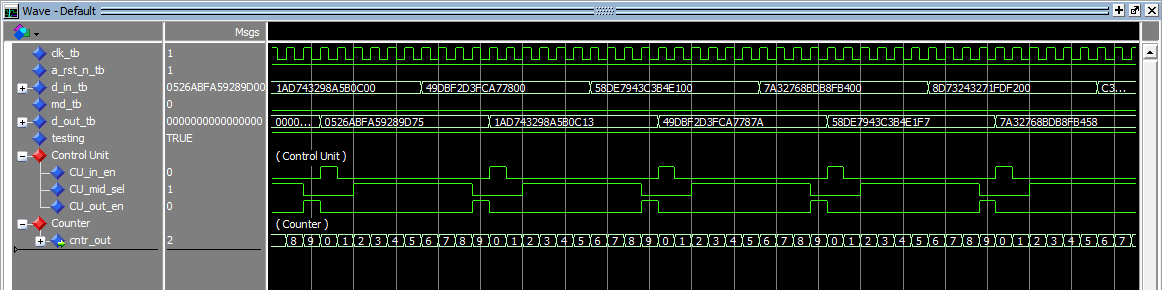
\includegraphics[scale=.6,clip]{img/test_lut_phase1.png}
    \end{center}
    \vspace*{-0.5cm}
    \caption{Testbench simulation of the LUT-based architecture (phase 1)}
    \label{fig:test_lut_phase1}
\end{figure}

\begin{figure}[H]
    \begin{center}
        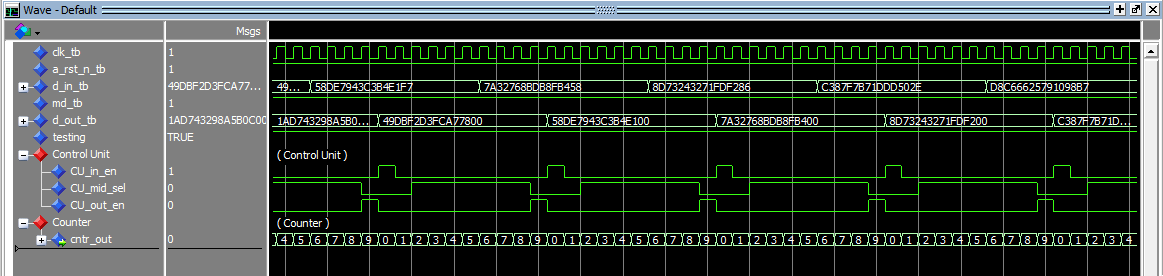
\includegraphics[scale=.6,clip]{img/test_lut_phase2.png}
    \end{center}
    \vspace*{-0.5cm}
    \caption{Testbench simulation of the LUT-based architecture (phase 2)}
    \label{fig:test_lut_phase2}
\end{figure}

\begin{figure}[H]
    \begin{center}
        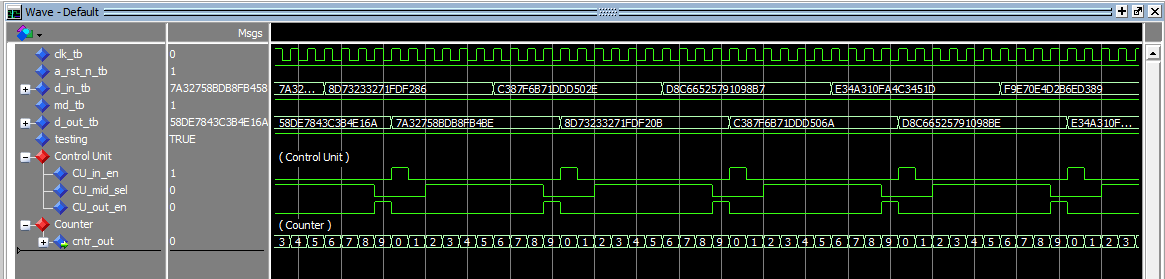
\includegraphics[scale=.6,clip]{img/test_lut_phase3.png}
    \end{center}
    \vspace*{-0.5cm}
    \caption{Testbench simulation of the LUT-based architecture (phase 3)}
    \label{fig:test_lut_phase3}
\end{figure}
%-------------------------------------------------------------------------------
% File: synth_results.tex
%
% Author: Marco Pinna
%         Created on 16/04/2022
%-------------------------------------------------------------------------------
\chapter{Synthesis results}\label{ch:synth_results}
This chapter concerns the automated logic synthesis process on the Xilinx Vivado Design Suite. The synthesis was performed using a Xilinx Zynq-7000 general purpose board (xc7z010clg400-1) as a target SoC.\\
Due to an insufficient number of I/O pins available on the actual board with respect to the ones requested by the specifications, the \textbf{implementation phase} was not carried out. Nevertheless, some results regarding resource usage, maximum clock frequency, critical path and power consumption could still be obtained during the synthesis phase.

\section{Bitwise architecture synthesis}
The synthesis process on Vivado showed no errors or warnings.\\

\subsection{Timing report}
After adding a time constraint for a clock period of 8 ns (125 MHz), the synthesis was re-run to obtain the timing report, whose summary is shown below:

\begin{figure}[H]
    \begin{center}
        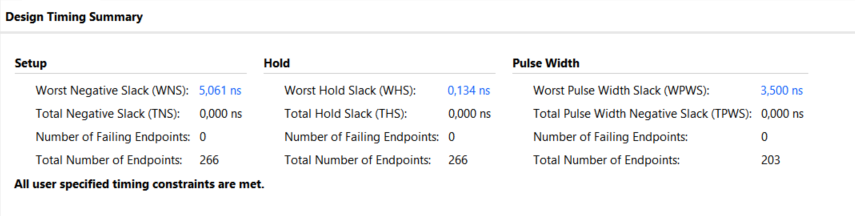
\includegraphics[scale=.75,clip]{img/vivado_bit_timing.png}
    \end{center}
    \vspace*{-0.5cm}
    \caption{Vivado timing report summary for the bitwise architecture synthesis}
    \label{fig:vivado_bit_timing}
\end{figure}

The Worst Negative Slack (WNS)is determined by the critical path of the circuit, which is highlighted in the figure below:

\begin{figure}[H]
    \begin{center}
        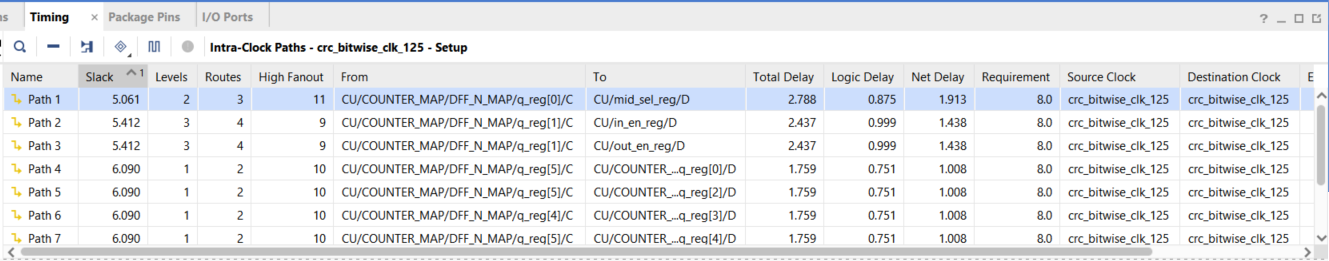
\includegraphics[scale=.5,clip]{img/vivado_bit_critical_path.png}
    \end{center}
    \vspace*{-0.5cm}
    \caption{Critical path of the bitwise architecture synthesis}
    \label{fig:vivado_bit_critical_path}
\end{figure}
\hfill \break
The figure shows that the critical path of the architecture is inside the Control Unit component.\\
Since the WNS has a positive value, this means that the board can be driven at a higher frequency than the one set in the timing constraints file.\\
The maximum allowed frequency can be computed with the following formula

\begin{equation}\label{eq:max_freq}
f_{max} = \frac{1}{T_{clk} - WSN} = \frac{1}{8 ns - 5,061 ns} = \frac{1}{2,939 ns} \approx 340,25 MHz
\end{equation}
\hfill \break
which is compatible with the 667 MHz maximum frequency stated in the board datasheet.\\
A simple computation can provide the throughput of the bitwise algorithm implementation: since every computation requires 58 clock cycles, the maximum number of CRCs that can be computed in a second is

\begin{equation}\label{eq:CRC_per_second}
R_{CRC} = \frac{f_{max}}{58} \approx 5866379
\end{equation}
\hfill \break
which, in terms of bit throughput, corresponds to approximately 328.52 Mbit/s.

\subsection{Resource utilization report}

The following figure shows a summary of the resource utilization report for the bitwise architecture.

\begin{figure}[H]
    \begin{center}
        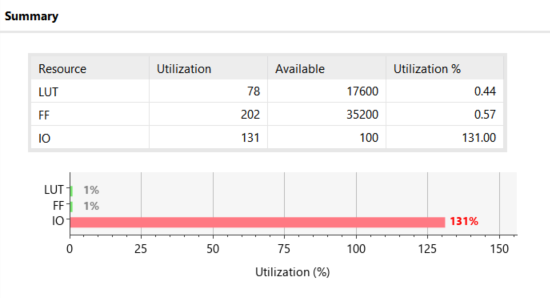
\includegraphics[scale=.75,clip]{img/vivado_bit_resources.png}
    \end{center}
    \vspace*{-0.5cm}
    \caption{Summary of the resource utilization report of the bitwise architecture}
    \label{fig:vivado_bit_resources}
\end{figure}
\hfill \break
As mentioned at the beginning of the chapter, the IO utilization exceeds 100\% since the specifications require a total of 131 ports while the IOB on the board amount to 100.\\
The LUT and FF utilization, on the other hand, is very low, standing at around 0.5\%.

\subsection{Power consumption report}

The following figure shows a summary of the power consumption utilization report for the bitwise architecture.

\begin{figure}[H]
    \begin{center}
        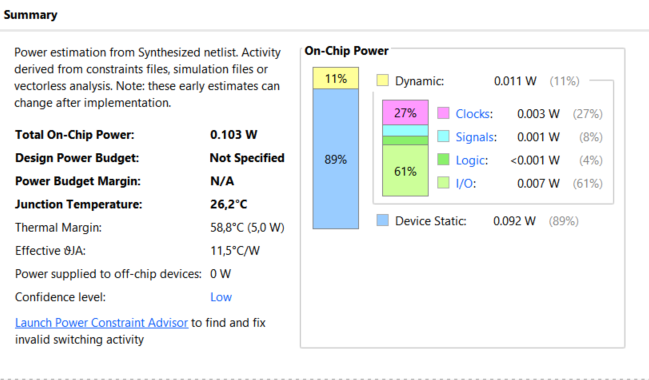
\includegraphics[scale=.85,clip]{img/vivado_bit_power.png}
    \end{center}
    \vspace*{-0.5cm}
    \caption{Summary of the power consumption report of the bitwise architecture}
    \label{fig:vivado_bit_power}
\end{figure}
\hfill \break
As it can be seen in the figure, the total power absorbed by the chip is around 0.1 W, most of which is static power consumption. This data however has to be taken with a grain of salt, since, as also stated in the figure, it has a low confidence level and the estimates could change after implementation.

\section{LUT-based architecture synthesis}
The same exact procedure was followed for the LUT-based architecture.\\
\hfill \break
The synthesis process on Vivado showed no errors or warnings.\\

\subsection{Timing report}
After adding a time constraint for a clock period of 8 ns (125 MHz), the synthesis was re-run to obtain the timing report, whose summary is shown below:

\begin{figure}[H]
    \begin{center}
        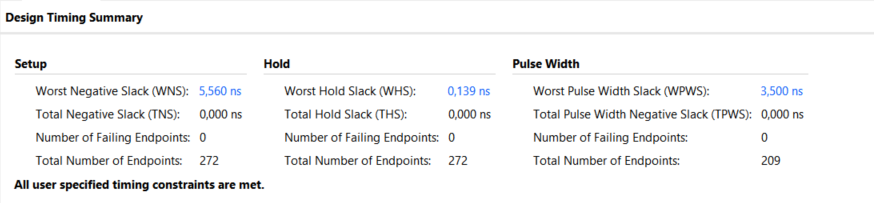
\includegraphics[scale=.75,clip]{img/vivado_lut_timing.png}
    \end{center}
    \vspace*{-0.5cm}
    \caption{Vivado timing report summary for the LUT-based architecture synthesis}
    \label{fig:vivado_bit_timing}
\end{figure}
\hfill \break
The Worst Negative Slack (WNS) has increased with respect to the bitwise architecture. The critical path of the circuit is highlighted in the figure below:

\begin{figure}[H]
    \begin{center}
        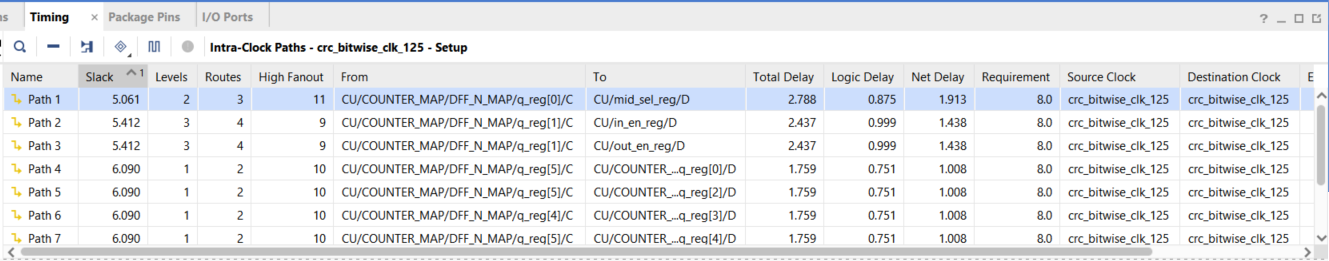
\includegraphics[scale=.5,clip]{img/vivado_bit_critical_path.png}
    \end{center}
    \vspace*{-0.5cm}
    \caption{Critical path of the bitwise architecture synthesis}
    \label{fig:vivado_bit_critical_path}
\end{figure}
\hfill \break
The figure shows that the critical path is now inside the PIPOShiftRegister.\\
Since in this case too the WNS has a positive value, this means that the board can be driven at a higher frequency than the one set in the timing constraints file.\\
Again, we can compute the maximum allowed frequency:

\begin{equation}\label{eq:max_freq}
f_{max} = \frac{1}{T_{clk} - WSN} = \frac{1}{8 ns - 5,560 ns} = \frac{1}{2,44 ns} \approx 409,84 MHz
\end{equation}
\hfill \break
which is higher than the other one and still compatible with the 667 MHz maximum frequency stated in the board datasheet.\\
\hfill \break
The throughput of the LUT-based algorithm implementation in terms of CRCs per second is:

\begin{equation}\label{eq:CRC_per_second}
R_{CRC} = \frac{f_{max}}{10} \approx 40984000
\end{equation}
\hfill \break
which, in terms of bit throughput, corresponds to approximately 2,295 Gbit/s.\\
The total speed-up from the bitwise implementation is about 600\%.

\subsection{Resource utilization report}

The following figure shows a summary of the resource utilization report for the LUT-based architecture.

\begin{figure}[H]
    \begin{center}
        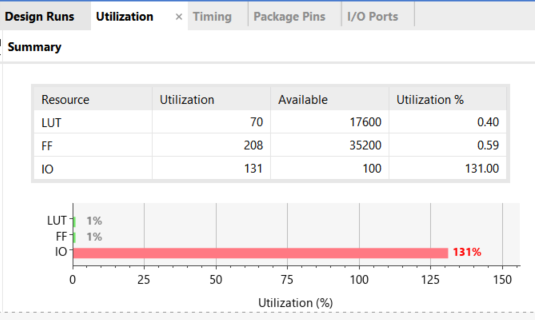
\includegraphics[scale=.75,clip]{img/vivado_lut_resources.png}
    \end{center}
    \vspace*{-0.5cm}
    \caption{Summary of the resource utilization report of the LUT-based architecture}
    \label{fig:vivado_bit_resources}
\end{figure}
\hfill \break
The report obviously present the same issue as before, as far as it concerns the IO utilization.\\
The LUT and FF utilization, surprisingly, are lower. This is thought to be a consequence of the optimizations performed by Vivado during the synthesis process.

\subsection{Power consumption report}

The following figure shows a summary of the power consumption utilization report for the LUT-based architecture.

\begin{figure}[H]
    \begin{center}
        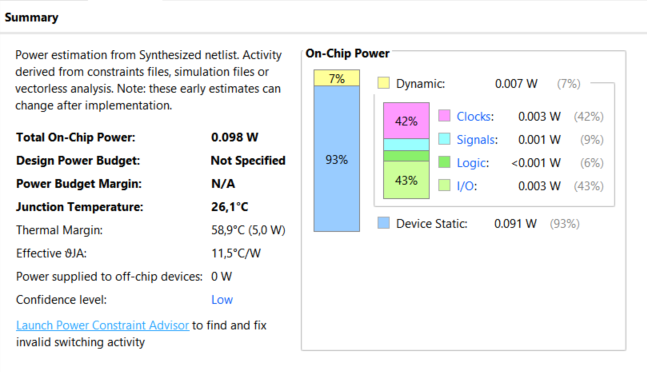
\includegraphics[scale=.85,clip]{img/vivado_lut_power.png}
    \end{center}
    \vspace*{-0.5cm}
    \caption{Summary of the power consumption report of the LUT-based architecture}
    \label{fig:vivado_bit_power}
\end{figure}

The total power absorbed by the chip is again in the order of 0.1 W, although slightly lower than the previous implementation. In this architecture too, most of it is static power consumption.\\
Just as before, this values should be taken with a grain of salt for the same reasons set forth.
%-------------------------------------------------------------------------------
% File: conclusions.tex
%
% Author: Marco Pinna
%         Created on 16/04/2022
%-------------------------------------------------------------------------------
\chapter{Appendices}\label{ch:conclusions}
%-------------------------------------------------------------------------------
% File: appendicies.tex
%
% Author: Marco Pinna
%         Created on <date>
%-------------------------------------------------------------------------------
\chapter{Appendices}

\end{document}
